\documentclass[aspectratio=169]{beamer}
\usepackage[utf8]{inputenc}
\usepackage{lmodern}
\usepackage{tikz}
\usepackage{hyperref}
\definecolor{pbprimary}{HTML}{D63031}
\definecolor{pbsecondary}{HTML}{FFE3E3}
\setbeamercolor{palette primary}{bg=pbprimary, fg=white}
\setbeamercolor{frametitle}{fg=pbprimary}
\setbeamercolor{title}{fg=pbprimary}
\setbeamercolor{block title}{bg=pbprimary, fg=white}
\setbeamercolor{block body}{bg=pbsecondary, fg=black}
\setbeamercolor{alertblock title}{bg=pbprimary, fg=white}
\setbeamercolor{alertblock body}{bg=pbsecondary!80, fg=black}
\setbeamertemplate{navigation symbols}{}
\setbeamertemplate{itemize item}{\color{pbprimary}\Large$\blacktriangleright$}
\title{FLEX Day : Possibly explore the Science Behind Pixaer website | or move into Business Project early to leave more time at the end of the year for All About Me Project}
\subtitle{Student Guide Deck}
\author{Pine Brook IGNITE}
\date{Spring 2026}
\begin{document}
\begin{frame}[plain]
\begin{center}
{\usebeamerfont{title}\color{pbprimary}\Huge FLEX Day : Possibly explore the Science Behind Pixaer website | or move into Business Project early to leave more time at the end of the year for All About Me Project\par}
\vspace{0.3cm}
{\Large Today we will learn, build, test, and show our thinking.\par}
\vspace{0.35cm}
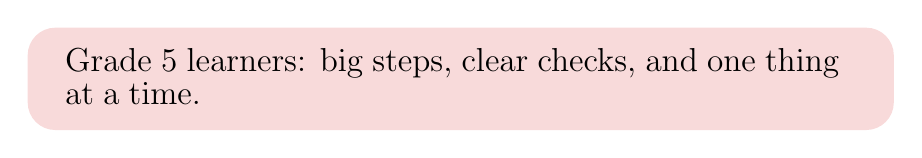
\begin{tikzpicture}
\fill[pbprimary!18, rounded corners=10pt] (0,0) rectangle (11,1.3);
\node[anchor=west, text width=10.2cm] at (0.35,0.68) {\large Grade 5 learners: big steps, clear checks, and one thing at a time.};
\end{tikzpicture}
\end{center}
\end{frame}
\begin{frame}{Todays Goal}
\begin{itemize}
\item Not listed
\end{itemize}
\begin{block}{Remember}
We do not have to be perfect right away. We take one step, then the next step, then we check.
\end{block}
\end{frame}
\begin{frame}{What You Need}
\begin{itemize}
\item Your class materials
\item The digital tool or build materials for today
\item A partner voice and your thinking
\end{itemize}
\begin{block}{Partner Norms}
Look. Listen. Try. Talk. Help without taking over.
\end{block}
\end{frame}
\begin{frame}{Step 1}
\begin{block}{Read todays goal and make a simple plan.}
Read todays goal and make a simple plan.
\end{block}
\begin{itemize}
\item Decide what you will finish first, next, and last.
\item Name the goal in student language before materials or devices create extra noise.
\end{itemize}
\centering\large\color{pbprimary} Pause. Check. Then move on.
\end{frame}
\begin{frame}{Step 2}
\begin{block}{Work through your checklist and pause for help when needed.}
Work through your checklist and pause for help when needed.
\end{block}
\begin{itemize}
\item Do not wait until the end to ask if you are stuck.
\item Keep one visible checklist or example on screen during work time.
\end{itemize}
\centering\large\color{pbprimary} Pause. Check. Then move on.
\end{frame}
\begin{frame}{Step 3}
\begin{block}{Share, reflect, or present your progress.}
Share, reflect, or present your progress.
\end{block}
\begin{itemize}
\item Be ready to explain one choice you made and why.
\item Pause once to help students reflect and reset before the final task push.
\end{itemize}
\centering\large\color{pbprimary} Pause. Check. Then move on.
\end{frame}
\begin{frame}{If You Get Stuck}
\begin{enumerate}
\item Read the directions on your screen or slide one more time.
\item Check the example, the checklist, or your partner role.
\item Try one small change before asking for a full rescue.
\item Students may lose the main goal if the task has too many moving parts.
\end{enumerate}
\begin{alertblock}{Help Routine}
Stop. Breathe. Point to where you are stuck. Ask a specific question.
\end{alertblock}
\end{frame}
\begin{frame}{Show Your Learning}
\begin{itemize}
\item I stayed with the steps and used the help routine when I needed it.
\item I made, coded, explained, or revised something that matches the lesson goal.
\item I can point to one choice, fix, or idea I learned today.
\end{itemize}
\begin{block}{Before You Leave}
Save it, share it, explain it, or demonstrate it.
\end{block}
\end{frame}
\begin{frame}{Teacher Voiceover Cues}
\footnotesize
\begin{itemize}
\item Today we are working on flex day : possibly explore the science behind pixaer website | or move into business project early to leave more time at the end of the year for all about me project. Watch first, then try it with me.
\item If you feel stuck, stop at the checkpoint slide and use the help routine before you panic.
\item Show what you learned by saving, sharing, explaining, or demonstrating one clear success move.
\end{itemize}
\color{gray}This slide can be removed before student use if you only want the visual deck.
\end{frame}
\end{document}
